\documentclass[DIV=8]{scrreprt}
\usepackage[czech]{babel}

\usepackage{amsmath}
\usepackage[version=4]{mhchem}
\usepackage{listings}
\usepackage{hyperref}
\newcommand{\inlinecode}{\texttt}
\graphicspath{{./resources/images/}}

%% Setup the fonts
\usepackage{tgpagella}
\usepackage{ebgaramond-maths}
\addtokomafont{labelinglabel}{\small\sffamily}

%% Setup the page layout
\usepackage{microtype} % micro adjustments to fonts
\usepackage{setspace} % set the line spacing
\onehalfspacing % the right 1.5 spacing between lines
\frenchspacing % no double space after full stop
\KOMAoptions{parskip=half} % no indentation of first lines, USA style
\recalctypearea

\usepackage{tikz}
\newcommand{\mybox}[2]{
    \paragraph{#1} #2
}
\lstset{
    basicstyle=\ttfamily,
    columns=fixed
}

\usepackage{etoolbox}
\makeatletter
\patchcmd{\scr@startchapter}{\if@openright\cleardoublepage\else\clearpage\fi}{}{}{}
\makeatother

\usepackage{enumitem}
\title{Strukturní biologie buňky}
\author{Evžen Wybitul \and Kateřina Krausová}

\begin{document}
\begin{titlepage}
\maketitle
\end{titlepage}
\tableofcontents


\marginline{Přednáška č. 1}

DNA má několik forem, konkrétně především B, A a Z. Tyto se liší velikostí žlábku, tvarem ribóz a případně orientací báze (synklinální/antiklinální).

\meta{Další informace též odpovídající část zápisů ze základů bioinformatiky (\href{https://eugleo.github.io/bioinformatika/doc/zaklady-bioinformatiky/notes.html\#Struktura\%20nukleových\%20kyselin}{DNA}, \href{https://eugleo.github.io/bioinformatika/doc/zaklady-bioinformatiky/notes.html\#Struktura\%20proteinů}{proteiny}) a také zápisy z \href{https://eugleo.github.io/bioinformatika/doc/biopolymery/notes.html}{celého druhého předmětu}.}

\section{Interakce mezi molekulami} \label{Interakce mezi molekulami} \FloatBarrier


Atomy (potažmo molekuly) jsou vázány kovalentně, nebo nekovalentně.

\paragraph{Nekovalentní vazby}
\begin{myItemize}[nosep]
    \item vodíkové můstky
\begin{myItemize}[nosep]
    \item interakce dvou elektronegativních atomů s jedním vodíkem
    \item délka 3Å
    \item s rostoucím úhlem klesá jejiich síla
    \item u proteinů energie \si{10 kJ/mol}
\end{myItemize}

    \item iontové interakce
    \item stacking interakce
\begin{myItemize}[nosep]
    \item vznikají kvůli \(\pi\) vazbám na aromatických sloučeninách
\end{myItemize}

    \item Van der Waalsovy interakce
\begin{myItemize}[nosep]
    \item působí mezi všemi páry atomů, které jsou v určité vzdálenosti
    \item přitažlivé
\end{myItemize}

    \item interakce kvůli hydrofobnímu efektu
\begin{myItemize}[nosep]
    \item přitažlivé (voda se snaží zachovat si co nejvíce vodíkových můstků)
    \item nejvíce mezi nepolárními sloučeninami
\end{myItemize}

\end{myItemize}



\section{Struktura proteinů} \label{Struktura proteinů} \FloatBarrier


\meta{Předpokládají se základní informace o proteinech a o stavbě a složení aminokyselin. Viz popříadě \href{https://eugleo.github.io/bioinformatika/doc/zaklady-bioinformatiky/notes.html\#Struktura\%20proteinů}{zápisky z bioinformatiky}.}

Proteiny jsou biopolymery složené z aminokyselin, které jsou vázané peptidickou vazbou. Peptidická vazba je ze 40\% rezonanční, a proto je planární; rotace je dovolena pouze kolem chirálních \(\ce{C\alpha}\). Volnost otáčení (tzv. torzní úhly) se zaznamnává na Ramachandranův diagram.

\paragraph{Stereoizomerie}
\begin{myItemize}[nosep]
    \item L a D forma AK (v těle je častější L)
\begin{myItemize}[nosep]
    \item buněčná stěna bakterií často obsahuje D formu, aby nebyly rozpoznány
\end{myItemize}

    \item většina AK (až na glycin) má chirální uhlík, proto stáčí rovinu polarizovaného světla
\end{myItemize}



\meta{L a D se dají "na papíře" jednoduše rozlišit; stačí najít chirální uhlík, zorientovat si jej vodíkem k sobě a poté sledovat, v jakém pořadí jsou jeho další vazební partneři. Pokud se ve směru hodinových ručiček dá přečíst pořadí \textbf{CO}, \textbf{R}, \textbf{N}, jedná se o \textbf{L formu}.}

\paragraph{Rotamery}
\begin{myItemize}[nosep]
    \item jednotlivé AK, které se liší pouze rotacemi kolem jednoduchých vazeb ve svém postranním řetězci
    \item existují knihovny rotamerů
\end{myItemize}



U proteinů rozlišujeme primární až kvartení strukturu.

\paragraph{Kvarterní struktura}
\begin{myItemize}[nosep]
    \item obligátní nebo neobligátní
\begin{myItemize}[nosep]
    \item obligátní = vyskytuje se jen v rámci daného "komplexu" a ne samostatně
\end{myItemize}

    \item symetrická a asymetrická (evolučně mladší)
    \item obvykle obsahuje malé množství podjednotek
\begin{myItemize}[nosep]
    \item výjimku tvoří F0ATPáza se 13 podjednotkami
\end{myItemize}

\end{myItemize}



\chapter{Nástroje} \label{Nástroje}


\marginline{Přednáška č. 2}

\paragraph{Přehled metod}
\begin{myItemize}[nosep]
    \item rentgenová krystalografie
\begin{myItemize}[nosep]
    \item difrakce RTG na elektronech
    \item nejpoužívanější
    \item nemá velikostní limit
\end{myItemize}

    \item NMR spektroskopie
\begin{myItemize}[nosep]
    \item využívá magnetické vlastnosti jader
    \item zkoumaná látka musí být v roztoku
    \item schopná zachytit i dynamiku molekul
    \item má velikostní limit
\end{myItemize}

    \item elektronová mikroskopie, cryoTEM
\begin{myItemize}[nosep]
    \item používá svazek elektronů s vysokou energií
    \item vhodná pro velké komplexy
    \item má nízké rozlišení
    \item kombinuje se s RTG a NMR strukturami
\end{myItemize}

    \item výpočetní metody
\begin{myItemize}[nosep]
    \item homologní modelování, strukturní bioinformatika
    \item není potřeba vzorek, vše je ale nutno porovnat s experimentálními daty
\end{myItemize}

\end{myItemize}



\section{Rentgenová krystalografie} \label{Rentgenová krystalografie} \FloatBarrier


\paragraph{Obecný postup}
\begin{myEnumerate}[nosep]
    \item příprava proteinu a krystalizace (dohromady kolem tří let)
    \item difrakční experiment
    \item vyřešení 3D struktury a její analýza
\end{myEnumerate}



\paragraph{Historie krystalů}
\begin{myItemize}[nosep]
    \item (1840) první proteinové krystaly: Hemoglobin, Hünefeld
\begin{myItemize}[nosep]
    \item víceméně omylem, kapali krev na sklíčko, molekuly vysychaly a praskly, vylil se z nich hemoglobin a zkrystalizoval
\end{myItemize}

    \item (1850) první metody krystalizace: Hemoglobin, Fünke
    \item (1909) The crystallography of Hemoglobins, Reichert Brown
\begin{myItemize}[nosep]
    \item cca 600 obrázků, hemoglobiny z různých živočišných druhů, na základě tvaru a velikosti krystalů se snažili evolučně propojit, jak jsou si různé druhy příbuzné
\end{myItemize}

    \item (1915) krystaly séra albuminu
    \item (1925) první krystal enzymu
    \item (1935) první krystal viru (tabáková mozaika)
\end{myItemize}



\paragraph{Historie RTG}
\begin{myItemize}[nosep]
    \item (1895) RTG záření, W. C. Röntgen
    \item (1910) teorie difrakce, Max von Laue
    \item (1912) difrakce na krystalu
    \item (1956) struktura myoglobinu, M. F. Perutz aj. C. Kendrew
\begin{myItemize}[nosep]
    \item viděli "párečky" (helixy)
\end{myItemize}

\end{myItemize}



RTG používáme místo běžného světla pro jeho kratší vlnovou délku; minimální rozlišení pozorování je totiž určeno jako \(D_{min} = \frac{\lambda}{2}\) (poté již dochází k ohybu světla). Pokud se chceme dostat na atomární rozlišení \si{1e10 m}, musíme používat RTG.

\subsection{Krystalizace proteinů} \label{Krystalizace proteinů}


Jedná se o nejtěžší část RTG krystalografie. Jako srážedla se používají soli, polymery, organické látky (odebírají proteinu vodu). Přesné krystalizační podmínky nelze předpovědět, proto se dělá \emph{screening} (testování 96 různých podmínek). Díky automatizaci je nyní možné na každý pokus vypotřebovat pouze malé množství proteinu.

\paragraph{Vlastnosti proteinových krystalů}
\begin{myItemize}[nosep]
    \item malé, symetrické
    \item většinou bezbarvé
    \item krychlová vnitřní struktura (shodná s diamantem, \(\ce{NaCl}\))
    \item malé styčné plochy, hodně prostoru mezi molekulami
\begin{myItemize}[nosep]
    \item kanály vyplněné krystalizační tekutinou (mateční roz­tok) tvoří až 70\% krystalu
\end{myItemize}

    \item struktura krystalu velmi připomíná nativní strukturu
\end{myItemize}



\paragraph{Faktory ovlivňující krystalizaci}
\begin{myItemize}[nosep]
    \item fyzikální
\begin{myItemize}[nosep]
    \item teplota, povrchy, doba krystalizace, gravitace, tlak, vibrace, elektrické a magnetické pole
\end{myItemize}

    \item chemické
\begin{myItemize}[nosep]
    \item pH, typ srážedla, koncentrace srážedla, iontová síla, specifické ionty, stupeň přesycení, koncentrace proteinu, neproteinové nečistoty
\end{myItemize}

    \item biochemické
\begin{myItemize}[nosep]
    \item čistota proteinu, ligandy, inhibitory, efektory, biologické zdroje, historie vzorku, stabilita proteinu, genetické modifikace, post- translační modifikace, chemické modifikace, isoelektrický bod
\end{myItemize}

\end{myItemize}



\subsection{Popis funkce} \label{Popis funkce}


\paragraph{Princip RTG krystalografie}
\begin{myEnumerate}[nosep]
    \item krystal ozařujeme RTG zářením
    \item výsledek vypadá jako odraz, ale je to difrakce
\begin{myItemize}[nosep]
    \item RTG interaguje s elektrony (předá jim energii), elektrony vyzáří sekundární vlnu
\end{myItemize}

    \item zaznamenáme intenzitu difrakce na detektor (kdysi fotografický papír, dnes elektronický detektor)
    \item provedeme Fourierovu syntézu (matematická operace)
    \item výsledkem je model proteinové struktury, konkrétně mapa elektronové hustoty
\end{myEnumerate}



\paragraph{Difrakční experiment}
\begin{myItemize}[nosep]
    \item na krystal pouštíme jeden zaostřený paprsek RTG o vybrané vlnové délce
    \item zaznamenáme difrakční obrazce ve všech směrech kolem krystalu
\end{myItemize}



\paragraph{Fourierova transformace}
\begin{myItemize}[nosep]
    \item matematická operace, díky níž můžeme spojitou funkci (s užitím Fourierovy analýzy) rozdělit na sadu periodických funkcí
    \item složky složíme zpět Fourierovou syntézou
    \item získáme tedy co, z čeho původně data vyšla, tedy mapu elektronové hustoty
\end{myItemize}



\paragraph{Fázový problém}
\begin{myItemize}[nosep]
    \item nejsme schopni získat fázi elektronové hustoty experimentálně
    \item máme několik metod, kterými ji zjišťujeme
\begin{myItemize}[nosep]
    \item metoda molekulového nahrazení: odhad na základě předchozích výsledků
    \item metoda anomálního rozptylu: zavedeme těžký kov (Se, Hg), do něj namočíme krystal, pak odhadujeme fázi
    \item metoda izomorfního nahrazení
\end{myItemize}

\end{myItemize}



Všechna PDB data jsou tedy pouze něčí interpretace mapy elektronové hustoty. Proto je také nyní povinnost ukládat do databází kromě struktury i původní strukturní data (tedy přesnou podobu experimentálních dat), aby si každý mohl interpretaci udělat sám.

\paragraph{Rozlišení}
\begin{myItemize}[nosep]
    \item závisí na kvalitě krystalu a intenzitě RTG záření
    \item do jakého úhlu jsme schopni zaznamenat difrakce
    \item nejlépe pod 2Å, neboť poté už hůře vidíme vodíkové můstky
\end{myItemize}



\section{Kryoelektronová mikroskopie} \label{Kryoelektronová mikroskopie} \FloatBarrier


Hodí se spíše pro větší vzorky; její rozlišení je omezené, ale stále se zlepšuje. V současné době se pohybuje kolem 6Å.

\paragraph{Postup}
\begin{myEnumerate}[nosep]
    \item vzorek vysušíme
\begin{myItemize}[nosep]
    \item ve vrstvě soli obsahující těžký atom (uranyl acetát)
    \item \emph{negativní barvení} (negative staining): zvýšení kontrastu, kontrola homogenity vzorku
\end{myItemize}

    \item umístíme jej na mřížku
    \item mřížku se vzorkem zmrazíme
\begin{myItemize}[nosep]
    \item v tekutém ethanu (cca 90°), rychlejší než dusík
\end{myItemize}

    \item umístíme mřížku do elektronového mikroskopu
    \item ozáříme mřížku proudem elektronů a sledujeme stíny částic
    \item vytvoříme 3D mapu rozmístění částic, z ní poté zhotovíme finální model
\end{myEnumerate}



\paragraph{Požadavky na vzorek}
\begin{myItemize}[nosep]
    \item velikost > \si{150 kDa} (čím větší, tím lepší)
    \item symetrie (oligomery)
    \item rigidita a stabilita
    \item homogenita (někdy lze ovšem rozlišit i více složek)
\end{myItemize}



Kromě toho je potřeba i vysokoenergetický dým s napětím \si{200} až \si{300 kV}.

\section{NMR spektroskopie} \label{NMR spektroskopie} \FloatBarrier

\marginline{Přednáška č. 3}

Nukleární magnetická rezonance se často používá v analytické chemii, kromě toho je ale užitečná i při zjišťování struktury proteinů.

\paragraph{Způsoby měření}
\begin{myItemize}[nosep]
    \item v kapalné fázi
\begin{myItemize}[nosep]
    \item vysokorozlišená a nízkorozlišená NMR (ta je jedna z nejpoužívanějších metod, je přesná)
\end{myItemize}

    \item v pevné fázi
\begin{myItemize}[nosep]
    \item druhá nejpoužívanější
    \item látky nesmí být v krystalu (vzorek musí být amorfní)
    \item vzorek je mikrokrystalický, nebo jeho molekuly tvoří agregáty
    \item vysokorozlišená NMR, širokopásmová NMR, mikroskopie
\end{myItemize}

    \item in vivo NMR
\begin{myItemize}[nosep]
    \item sledování buněk a živých tkání
    \item MR imaging
\end{myItemize}

\end{myItemize}



\paragraph{Předměty studia}
\begin{myItemize}[nosep]
    \item prostorové uspořádání molekul (statický obraz)
    \item vzájemné interakce
\begin{myItemize}[nosep]
    \item zásadní pro strukturní biologii
\end{myItemize}

    \item dynamické chování molekul
\begin{myItemize}[nosep]
    \item na úrovni postranních řetězců, celých molekul nebo domén
    \item vhodná pro pozorování dějů trvajících mikrosekundy, nanosekundy
\begin{myItemize}[nosep]
    \item čím jsou molekuly pomalejší, tím méně je NMR vhodná
\end{myItemize}

\end{myItemize}

\end{myItemize}



\paragraph{Princip funkce}
\begin{myItemize}[nosep]
    \item jádra mají spin (otáčejí se), a náboj -> chovají se jako magnety
\begin{myItemize}[nosep]
    \item konkrétně musí ještě mít lichý počet neutronů a/nebo protonů
    \item když je vložíme do magnetického pole, budou se nějak orientovat
\end{myItemize}

    \item na NMR měříme, kolik energie musíme vynaložit na to, aby se jádra přesunula do rezonančního stavu (jejich magnetické pole se vychýlí přesně proti vnějšímu magnetickému poli)
\begin{myItemize}[nosep]
    \item tato energie je ovlivněna počtem elektronů v blízkosti atomu
    \item přesunu do rezonančního stavu se říká \emph{precesní pohyb}, má konkrétní frekvenci a potřebnou energii pro konkrétní jádro v konkrétním elektronovém kontextu
\end{myItemize}

    \item energii dodáme atomům pomocí radiofrekvenčního vysílače
\begin{myItemize}[nosep]
    \item po vypnutí se atomy vrátí do původní polohy
    \item tento pohyb indukuje v cívce proud, který zpracujeme jako NMR signál
\end{myItemize}

    \item odezvu (měření rezonančních frekvencí jednotlivých atomů) měříme v závislosti na čase a analyzujeme ji pomocí Fourierovy transformace
\end{myItemize}



NMR malých molekul je základním nástrojem analytické chemie. V naměřených spektrech je ale více signálů a šířka čar odráží velikost systému. U komplikovanějších molekul, kde dochází k překryvu signálů, je třeba použít vícedimenzionální spektra a/nebo NMR aktivní heterojádra.

NMR biomolekul velice závisí na velikosti těchto molekul; čím je molekula větší, tím pomaleji se v roztoku pohybuje. A pomalé rotace vedou k rozšiřování čar signálů. To je zároveň \textbf{největší nevýhoda NMR}: systém musí být jen tak veliký, aby čáry signálů nepřesáhly šířku, za kterou už je nemůžeme analyzovat.

\paragraph{Zdroj magnetického pole}
\begin{myItemize}[nosep]
    \item magnet (ve tvaru nádoby)
    \item supravodivá cívka chlazená héliem, na ní několik plášťů (mezi nimi vakuum kvůli izolaci), další kryokapaliny (dusík)
\begin{myItemize}[nosep]
    \item musí být ve stabilním prostředí, je nutné neustále doplňovat kapaliny
\end{myItemize}

    \item samotná nádoba má průměr asi \si{2 m}
    \item uprostřed cívky je šachta, zespoda sonda
\begin{myItemize}[nosep]
    \item k sondě je nutné přivést radiofrekvenční záření
\end{myItemize}

\end{myItemize}



\subsection{NMR proteinů} \label{NMR proteinů}


Právě u proteinů se objevuje problém s citlivostí NMR.

\paragraph{Metody pozorování}
\begin{myItemize}[nosep]
    \item proteiny jsou velké, rotují pomalu, jejich NMR signály jsou široké
    \item komplexní a repetitivní sekvence způsobují překryvy čar
    \item čím vyšší energii bude mít použité záření, tím necitlivější naše metoda bude
    \item \(\ce{^12C}\) ani \(\ce{^14N}\) nejde na NMR vidět, musí se proto substituovat \(\ce{^13C}\) a \(\ce{^15N}\)
\begin{myItemize}[nosep]
    \item stavíme \emph{korelační mapu}, kde zjišťujeme korelaci mezi protony a dusíky a korelaci mezi protony a uhlíky
\end{myItemize}

\end{myItemize}



\meta{Následující odstavec prý zcela jistě bude ve zkouškovém testu.}
Narozdíl od RTG krystalografie pozorujeme u NMR \textbf{přímou odezvu konkrétních atomů a skupin}, z těchto jednoduchých dat poté můžeme sestavit model popisující interakce těchto částí. Jedná se tedy o \textbf{přímé porovnání}.

\paragraph{Postup získání strukturní informace}
\begin{myEnumerate}[nosep]
    \item přiřazení signálu jednotlivým skupinám a atomům
    \item získání strukturních omezení
\begin{myItemize}[nosep]
    \item intenzita signálu klesá se vzdáleností (s šestou mocninou)
    \item nevidíme přes helixy
\end{myItemize}

    \item tvorba matice strukturních zobrazení
\begin{myItemize}[nosep]
    \item soubor konformací vyhovujících omezením
\begin{myItemize}[nosep]
    \item pouze upřesnění modelu, ne přesný výpočet
    \item na periferiích jsou větší omezení
\end{myItemize}

    \item vypadá jako mapa elektronové hustoty
    \item nejprve se skládají lokální části
\end{myItemize}

\end{myEnumerate}



\section{Biomolekulární hmotnostní spektrometrie} \label{Biomolekulární hmotnostní spektrometrie} \FloatBarrier


\begin{myItemize}[nosep]
    \item pozorujeme složení, stechiometrii, vazbu malých molekul, homogenitu, čistotu
    \item vidíme spektra s atomárním rozlišením, zjistíme co je na molekulu připojeno (různé modifikace)
    \item jsme schopni separace podle iontové mobility
    \item velmi cenná v kombinaci s krystalografií
\end{myItemize}



\paragraph{Princip funkce}
\begin{myItemize}[nosep]
    \item potřebujeme molekuly převést do plynné fáze a z neutrálního stavu je dostat do iontového
\begin{myItemize}[nosep]
    \item ESI (electrospray ionization), MALDI (matrix- assisted laser desorption/ionization)
\end{myItemize}

    \item molekuly prochází přes spektrometr
\begin{myItemize}[nosep]
    \item v plynné fázi prochází přes vlastní spektrometr, který má více úseků
    \item je vhodné použít i jiné způsoby dělení
\end{myItemize}

    \item na základě velikosti a náboje se molekuly oddělí a my je snímáme na hmotnostních spektrech
\begin{myItemize}[nosep]
    \item vzniká více čar, kde každá odpovídá jednomu náboji
    \item z toho lze zjistit, jak daný komplex vypadá a jaké má složení
\end{myItemize}

\end{myItemize}



\paragraph{Předměty studia}
\begin{myItemize}[nosep]
    \item velice podobné NMR
    \item chemický crosslinking
    \item výměna vodíku za deuterium (\textbf{HDX}, hydrogen-deuterium exchange)
    \item prostorové uspořádání molekul
    \item vzájemné interakce
    \item dynamické chování interakcí
\end{myItemize}



\paragraph{HDX experiment}
\begin{myItemize}[nosep]
    \item protein se dá do \(\ce{D2O}\), tedy vody, kde je vodík nahrazen deuteriem
    \item deuterium proniká do proteinu (vyměňuje se s vodíkem na páteři proteinu), protein je těžší
    \item rychlost výměny \(\ce{D <-> H}\) závisí na tom, jestli má protein v daném místě navázaný ligand (pokud ano, je pomalejší)
    \item stačí tedy změřit rychlost HDX s různými ligandy (globální HDX), popřípadě je možné protein rozsekat proteázou a změřit HDX u každého kousku
\begin{myItemize}[nosep]
    \item z toho zjistíme, která část proteinu váže jaký ligand
    \item používá se LC-MS (kapalinová chromatografie s hmotnostním spektrometrem)
\end{myItemize}

\end{myItemize}



\section{Bioinformatika (výpočetní metody)} \label{Bioinformatika (výpočetní metody)} \FloatBarrier


Výpočetní metody studují stejné problémy jako NMR a hmotnostní spektrometrie: prostorové uspořádání molekul, jejich dynamické chování a vzájemné interakce.

\meta{Další informace lze najít v oddílu \href{https://eugleo.github.io/bioinformatika/doc/zaklady-bioinformatiky/notes.html\#Predikce\%20struktury}{predikce struktury}.}

\paragraph{Dělení}
\begin{myItemize}[nosep]
    \item homologní modelování
\begin{myItemize}[nosep]
    \item na základě podobnosti v sekvenci
    \item jsme schopni porovnat primární sekvence molekul jako takové
    \item počty struktur jsou veliké, chemický prostor je už ale dobře mapován, proto jsme schopni vyřešit minimálně části proteinů
    \item podobnost velmi vysoká
\end{myItemize}

    \item ab initio metody
\begin{myItemize}[nosep]
    \item de novo návrh struktur
    \item Rosetta
\end{myItemize}

    \item MD simulace, hybridní modelování
\begin{myItemize}[nosep]
    \item folding, molecular docking
    \item simulace pohybů na časových škálách, které neumíme pozorovat jinými metodami
\end{myItemize}

\end{myItemize}



\paragraph{Základní principy}
\begin{myItemize}[nosep]
    \item srovnáme sekvence, hledáme homologii
\begin{myItemize}[nosep]
    \item pokud nalezneme, můžeme zjistit sekvenci, strukturu
    \item pokud ne, musíme přistoupit k tvoření ab initio
\end{myItemize}

    \item ab initio výpočet struktury
\begin{myItemize}[nosep]
    \item velký problém s parametrizací
    \item Rosetta (David Baker)
\begin{myItemize}[nosep]
    \item vychází ze známých pdb struktur rozsekaných na malé fragmenty
    \item porovnává sekvence, skládá fragmenty a hádá, jak by mohla vypadat další sekvence
    \item poté vybere model a provede validaci
\end{myItemize}

\end{myItemize}

    \item simulace molekulární dynamiky (MD simulation)
\begin{myItemize}[nosep]
    \item je používána homologním modelováním i ab initio metodami
    \item poskytuje různá rozlišení
    \item slouží k testování strukturního efektu mutací (např. u HIV reverzní transkriptázy)
\end{myItemize}

    \item konstrukce hybridních strukturních modelů
\begin{myItemize}[nosep]
    \item umožňuje integrovat informace z různých metod
\end{myItemize}

\end{myItemize}



\chapter{Enzymy} \label{Enzymy}

\marginline{Přednáška č. 4}

\begin{myItemize}[nosep]
    \item oxidoreduktázy (přenášejí \(\ce{H+}\) nebo \(\ce{O}\))
    \item transferázy
    \item hydrolázy
    \item lyázy
    \item isomerázy
    \item ligázy
\end{myItemize}



\paragraph{Mechanismus funkce}
\begin{myItemize}[nosep]
    \item funkce je ovlivněná strukturou
    \item váží se na substrát a snižují energetickou bariéru, takže reakce může proběhnout rychleji
    \item mechanismus zámku a klíče
\begin{myItemize}[nosep]
    \item enzym má preformované aktivní místo, do kterého se vejde pouze jeden substrát s určitými vlastnostmi
    \item pouze pro tento substrát reakce proběhne
\end{myItemize}

    \item mechanismus induced fit (indukovaného přizpůsobení)
\begin{myItemize}[nosep]
    \item aktivní místo nemusí být připravené na daný klíč
    \item na enzym se může navázat substrát, který indukuje změnu vazebného místa
    \item hexokináza: po vazbě obou substrátů se aktivní místo přizpůsobí tak, že reakce může proběhnout
\end{myItemize}

    \item některé enzymy potřebují "pomocníky"
\begin{myItemize}[nosep]
    \item kofaktory
    \item koenzymy
    \item prostetické skupiny
    \item allosterické regulátory (molekuly vázající se mimo aktivní místo)
\end{myItemize}

\end{myItemize}



\paragraph{Inhibitory}
\begin{myItemize}[nosep]
    \item kompetitivní
\begin{myItemize}[nosep]
    \item přímo se váží na aktivní místo
    \item kompetují se substrátem
\end{myItemize}

    \item nekompetitivní
\begin{myItemize}[nosep]
    \item váží se mimo aktivní místo
\end{myItemize}

\end{myItemize}



\section{Karbonátlyáza} \label{Karbonátlyáza} \FloatBarrier


\begin{myItemize}[nosep]
    \item anglicky carbonic anhydrase (CA)
    \item katalyzuje reakci
\[\ce{CO2 + H2O <=> H+ + HCO3-}\]
\begin{myItemize}[nosep]
    \item tato reakce je samovolná
\end{myItemize}

    \item nejrychlejší enzym na světě, hydratuje \(10^6\) molekul \(\ce{CO2}\) za sekundu (zrychluje reakci \(10^7\) krát)
    \item pět tříd: \(\alpha, \beta, \gamma, \delta, \zeta\) (a nově objevená šestá třída \(\eta\))
\begin{myItemize}[nosep]
    \item všechny mají jako kofaktor nějaký kov (\(\ce{Zn}\), \(\ce{Mo}\), \(\ce{Cd}\))
    \item v těle máme \(\alpha\)
\end{myItemize}

\end{myItemize}



\todo{Vysvětlit, jak přesně se zinek účastní enzymatické reakce.}

\paragraph{Zinečný kofaktor}
\begin{myItemize}[nosep]
    \item konkrétně \(\ce{Zn^{2+}}\)
    \item je koordinován histidinovými zbytky
    \item koordinuje vodu, snižuje pKa vody na 7
    \item stará se o odštěpení protonu
    \item hydroxid zůstane navázaný na iontu, přichází substrát, dochází k nukleofilnímu ataku, odchází produkt a celá reakce pokračuje
\end{myItemize}



\subsection{Lidské CA} \label{Lidské CA}


\begin{myItemize}[nosep]
    \item pomáhají udržovat acidobazické prostředí v organizmu
    \item účastní se \(\ce{CO2}\) a \(\ce{HCO3}\) transportu
\begin{myItemize}[nosep]
    \item respirace, resorpce kostí, glukoneogeneze, urogeneze, lipogeneze
\end{myItemize}

    \item 16 izoforem
\begin{myItemize}[nosep]
    \item CAII
\begin{myItemize}[nosep]
    \item ve všech buňkách, je jí hodně
    \item je stabilní, dobře krystalizuje
    \item má dobře definované aktivní místo, od něj vede cestička k C konci vystlaná His
    \item slouží jako off target: často chceme cílit léky na CAIX, ale zároveň nechceme inhibovat žádné její isoformy (to se právě těstuje na CAII)
\end{myItemize}

    \item CAIX: nadprodukce u nádorů, marker rakoviny, cíl vyvíjených léků
\end{myItemize}

\end{myItemize}



\paragraph{Inhibitory CA}
\begin{myItemize}[nosep]
    \item známe strukturu CA => místo substrátu můžeme navrhnout kompetitivní inhibitor
\begin{myItemize}[nosep]
    \item např. sulfanomid
\end{myItemize}

    \item inhibitory lidské CA
\begin{myItemize}[nosep]
    \item všech 16 izoforem si je velice podobných
    \item CAII anti-glaucoma drugs (glaukom je zelený zákal)
    \item CAV je cílem léků proti obezitě
    \item CAVII je v mozku, je cílem léků na bolest hlavy a epilepsii
\end{myItemize}

\end{myItemize}



\paragraph{Strukturou inspirované inhibitory}
\begin{myItemize}[nosep]
    \item cesta od ihibitoru k léku je drahá a dlouhá
    \item pokud známe enzym a jeho inhibitor (a určíme jejich strukturu), můžeme inhibitor upravit tak, aby se vázal lépe (specifičtěji, s větší afinitou)
\begin{myItemize}[nosep]
    \item jedná se o iterativní proces vývoje z lead structure do finální struktury, která poté může jít do klinických testů
\end{myItemize}

\end{myItemize}



\section{HIV proteáza} \label{HIV proteáza} \FloatBarrier


Enzym vyskytující se v retroviru HIV. V buňce se přepíše z RNA do DNA. Je jedním z hlavních cílů pro léky HIV.

\paragraph{Struktura}
\begin{myItemize}[nosep]
    \item zcela symetrický dimer
    \item dva řetězce, dvě podjenotky; každý řetězec je složek z 99 AK
    \item obě podjednotky jsou u sebe drženy svými N a C konci, kromě toho také aktivním místem ("zakousnou" se do sebe)
    \item v aktivním místě jsou Asp (podobně jako u pepsinu)
\end{myItemize}



\paragraph{Funkce}
\begin{myItemize}[nosep]
    \item štěpí polyprotein na jednotlivé proteiny nutné k fungování viru
\begin{myItemize}[nosep]
    \item klíčová pro správnou funkci viru
\end{myItemize}

    \item pro katalýzu je důležitá molekula vody
    \item aktivní místo nemá předpřipravené, vytvoří se až po navázání substrátu (induced fit)
\begin{myItemize}[nosep]
    \item po navázání substrátu vypudí všechnu přebytečnou vodu
\end{myItemize}

    \item je \emph{promiskuitní}, rozpoznává celou řadu substrátů (devět)
    \item na začátku musí rozštěpit i sebe
\end{myItemize}



Podle tvaru substrátu se vyvinula léčiva, která funkci enzymu inhibují (např. ritonavir). Deset takových inhibitorů je v klinické praxi; virus ale díky reverzní transkripci, která často chybuje, velice rychle mutuje a rychle si vyvine proti léčivu rezistenci. Tyto (primární) mutace často musí být kompenzovány mutacemi sekundárními.

\begin{description}
\item[primární mutace]\hfill \\
Snižují afinitu k inhibitoru, vyskytují se především na aktivním místě.


\item[sekundární mutace]\hfill \\
Kompenzují efekt primárních mutací na aktivitu, zaručují, že primární mutace nebudou mít na aktivitu negativní dopad. Vyskytují se dále od aktivního místa.

\end{description}


\section{ATP syntáza} \label{ATP syntáza} \FloatBarrier


\begin{myItemize}[nosep]
    \item v membráně mitochondrií, chloroplastů a bakterií
    \item katalyzuje reakci
\[\ce{ADP + Pi + H_{out} <=> ATP + H2O + H_{in}}\]
\begin{myItemize}[nosep]
    \item syntetizuje ATP z ADP a fosfátu, využívá k tomu protonový gradient
\end{myItemize}

    \item dodává všem organizmům energii
    \item funguje trochu jako molekulární motor: \(\ce{F0}\) podjednotku v membráně pohání protony, zatímco \(\ce{F1}\) podjednotku pohání ATP
    \item \(\ce{F0}\) podjednotka se dá inhibovat oligomycinem
\end{myItemize}



\chapter{Membrány} \label{Membrány}


\begin{myItemize}[nosep]
    \item zajišťují tvar buněk, komunikaci, obranu, přichycení, rozpoznávání a přenos signálů
    \item urdžují specifické prostředí buňky: koncentraci iontů, malých metabolitů a makromolekul
    \item eukaryota mají membrány i uvnitř buňky
    \item složení
\begin{myItemize}[nosep]
    \item lipidová dvojvrstva
    \item proliny
    \item glycerocalyx, "cukerný obal"
    \item steroly vložené v lipidové dvojvrstvě
\end{myItemize}

    \item velmi dynamická struktura --- model fluidní mozaiky
    \item cytoplazmatická část je negativnější než exoplazmatická
\end{myItemize}



\paragraph{Tloušťka membrány}
\begin{myItemize}[nosep]
    \item nemá konstantní tloušťku
\begin{myItemize}[nosep]
    \item záleží na typu membrány, teplotě apod.
    \item v literatuře \(4\) až \si{10 nm}, obvykle \(5\) až \si{6 nm}
\end{myItemize}

    \item \si{3 nm} hydrofobní jádro a \(1\) až \si{1,5 nm} polární hlavy
    \item apikální membrána jaterní buňky je asi o 7Å širší než basolaterální membrána
    \item membrána v uspořádaném stavu (nižší teplota) je užší než v neuspořádaném stavu
    \item ohyby membrány způsobeny složením lipidů a proteinů (fosfatidylcholin a sfingomyelin způsobují konvexní pohyb)
\end{myItemize}



\section{Lipidy} \label{Lipidy} \FloatBarrier


Lipidů je až 200 typů.

\paragraph{Glycerofosfolipidy}
\begin{myItemize}[nosep]
    \item nejčastější
    \item glycerol + 2 alifatické řetězce
\begin{myItemize}[nosep]
    \item jeden zahnutý (nenasycený), druhý přímý (nasycený)
\end{myItemize}

    \item přes esterovou vazbu návázán fosfátový zbytek a další alkohol
    \item různé typy se liší v navázaném alkoholu
    \item některé fungují jako signální
\end{myItemize}



\paragraph{Sfingolipidy}
\begin{myItemize}[nosep]
    \item často v mozku
    \item účastní se zánětlivých reakcí
    \item často v části směřující do extracelulárního prostoru
\end{myItemize}



\paragraph{Steroly}
\begin{myItemize}[nosep]
    \item 20-- 30\% všech membrán
    \item Produkují se v obrovském množství (1--2g/den/člověk)
    \item ovlivňují tekutost (fluiditu) membrány (mohou zvyšovat i snižovat)
    \item nezbytná součást membrán
    \item polarizované
    \item aromatické kruhy a OH skupina
    \item např. cholesterol
\end{myItemize}



\paragraph{Ethery}
\begin{myItemize}[nosep]
    \item díky nim mohou archea přežívat i v extrémních podmínkách
\end{myItemize}



\paragraph{Distribuce lipidů na membráně}
\begin{myItemize}[nosep]
    \item lipidy jsou na membráně distribuovány asymetricky, vznikají \textbf{lipidové rafty}
\begin{myItemize}[nosep]
    \item ostrůvky bohaté na proteiny, membránové mikrodomény
    \item vznik po laterálním pohybu proteinů
    \item organizační centra pro uspořádávání signálních makromolekuul
    \item ovlivňují membránovou fluiditu a transport membránových proteinů
    \item regulují neurotransmisi
\end{myItemize}

    \item enzymy schopné přehazovat lipidy na druhou stranu vrstvy
\begin{myItemize}[nosep]
    \item flipázy, flopázy, skramblázy
\end{myItemize}

\end{myItemize}



\section{Membránové proteiny} \label{Membránové proteiny} \FloatBarrier


Většina léků je založena na interakci s membránovými proteiny.

\paragraph{Tvary}
\begin{myItemize}[nosep]
    \item sedminásobný helix
    \item beta barel
    \item periferální
    \item zanořený alfa helix
\end{myItemize}



\begin{description}
\item[prenylace]\hfill \\
Připojení isoprenoidů (např. farnesylu, geranyl-geranylu) k cysteinům cílového proteinu.


\item[mytistoylace]\hfill \\
Druh acylace. Připojení zbytku kyseliny myristové ke koncovému glycinu proteinu.


\item[palmitoylace]\hfill \\
Druh acylace. Připojení zbytku kyseliny palmitové na \(\ce{SH}\) skupinu cysteinu.

\end{description}


\paragraph{Proteiny asociované s lipidy}
\begin{myItemize}[nosep]
    \item kovalentní interakce
    \item periferální proteiny
    \item způsoby připojení
\begin{myItemize}[nosep]
    \item prenylace, acylace (mytistoylace, palmitoylace)
    \item připojení pomocí GPI kotvy (přes glykofosfatidylinositol)
\end{myItemize}

\end{myItemize}



\begin{description}
\item[positive inside rule]\hfill \\
Intracelulární rezidua mají kladnější náboj než ta extracelulární. Souvisí to se záporným nábojem vnitřní strany mebrány. Tento jev se využívá při predikci orientace proteinu.

\end{description}


S tímto pravidlem souvisí také jev tzv. "šnorchlování", což je interakce polárních skupin proteinů s polárními skupinami lipidů hluboko v membráně.

\subsection{Primární struktura} \label{Primární struktura}


\begin{myItemize}[nosep]
    \item aminokyselinové složení odlišné od ostatních proteinů
\begin{myItemize}[nosep]
    \item relativně vysoký obsah Gly a Pro
    \item vysoké zastoupení Tyr a Trp (3x vyšší než u cytosolických proteinů)
    \item vysoké zastoupení Lys a Arg v cytoplazmatické části (smyčky)
\end{myItemize}

    \item ze sekvence lze z 98\% určit, zda se jedná o membránový protein či ne
    \item výrazně hydrofobní transmembránové (TM) úseky o délce okolo 20AK
\end{myItemize}



\subsection{Sekundární struktura} \label{Sekundární struktura}


\paragraph{Proline kink}
\begin{myItemize}[nosep]
    \item zlom na helixu způsobený proliny
    \item okolo zlomu jsou časté Ser a Thr
    \item prolin dělá ostrou zatáčku v membráně
\begin{myItemize}[nosep]
    \item někdy vhodné pro regulační vlastnosti, někdy pro přizpůsobení se
    \item může zvětšit flexibilitu toho, co je třeba navázat
\end{myItemize}

\end{myItemize}



\paragraph{Reentrant loops}
\begin{myItemize}[nosep]
    \item helix neprojde skrz celou membránu, ale otočí se a vyjde tam, kde vešel
    \item obsahuje je 10\% membránových proteinů
    \item s rostoucím počtem TM úseků roste pravděpodobnost výskytu
\end{myItemize}



\paragraph{Experimentální určení struktur}
\begin{myItemize}[nosep]
    \item náročné --- potřebujeme protein vyizolovat a dostat do roztoku
    \item průlomem bylo objevení detergentů a kryoelektronové mikroskopie
    \item detergenty
\begin{myItemize}[nosep]
    \item citlivě rozrušují membránu
    \item obalí hydrofobní části
\end{myItemize}

    \item MemProtMD
\begin{myItemize}[nosep]
    \item databáze struktur membránových proteinů
    \item 150 000 struktur, z toho 3000 membránové proteiny
    \item první struktura 1982
\end{myItemize}

\end{myItemize}



\subsection{Příklady membránových proteinů} \label{Příklady membránových proteinů}


\paragraph{Poriny}
\begin{myItemize}[nosep]
    \item objeveny v bakteriích, u eukaryot se nalézají v mitochondrální membráně
    \item kanály tvořící v membrně pór
    \item v kanálu často váží vápenaté ionty, jsou zde často kladně nabité
    \item častý je trimerní porin
\begin{myItemize}[nosep]
    \item tři díry ve specifické orientaci
    \item není většinou příliš specifický
\end{myItemize}

\end{myItemize}



\paragraph{G-protein-coupled receptors}
\begin{myItemize}[nosep]
    \item receptory spřažené s G-proteiny
    \item struktura G-proteinu objevena roku 2007, struktura G-proteinu v komplexu objevena roku 2011
    \item více viz \hyperref[G-protein-coupled receptors]{oddíl o GPCR} v tomto textu
\end{myItemize}



\paragraph{Draselný kanál}
\begin{myItemize}[nosep]
    \item tetramer: čtyři podjednotky, tři slabiky, dva transmembránové helixy, jeden otvor
    \item úzký průchod, extrémně selektivní --- prochází pouze draslík
\begin{myItemize}[nosep]
    \item sodík je sice menší, a měl by tedy procházet také, ale draslík se umí lépe zbavit vody --- na rozdíl od sodíku, který proto kanálem neprojde
\end{myItemize}

    \item karboxylové skupiny draslík dobře koordinují
\end{myItemize}



\paragraph{Sting}
\begin{myItemize}[nosep]
    \item aktivátor a stimulátor genů
    \item nachází se v membránách ER
    \item má imunitní povahu, spouští protizánětlivou reakci při styku s cizí DNA
    \item po navázání cAMP dochází k otočení transmembránové části o 180\(^{\circ}\)
\end{myItemize}



\paragraph{Bakteriální ATP syntáza}
\begin{myItemize}[nosep]
    \item enzym produkující ATP
    \item byla za něj udělena Nobelova cena
    \item struktura nebyla určena celá
\end{myItemize}



\paragraph{Kardiolipin}
\begin{myItemize}[nosep]
    \item tvoří až 20\% fosfolipidů
\end{myItemize}



\chapter{Struktura DNA} \label{Struktura DNA}


Většina strukturních informací je z elektronové mikroskopie.

\begin{figure}
    \caption{Obrázek makrostruktury DNA}
    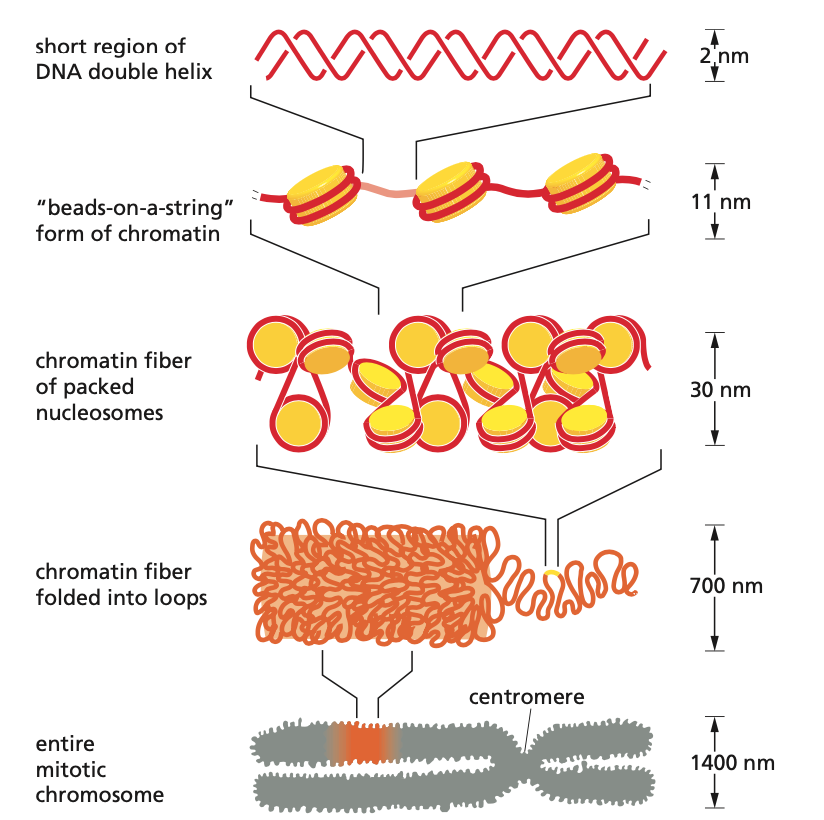
\includegraphics[width=0.85\textwidth]{dna_makrostructure.png}
    \centering
    \label{}
\end{figure}



\paragraph{Makrostruktura DNA}
\begin{myItemize}[nosep]
    \item do \si{5 \mu m} je potřeba složit více než metr DNA, proto je DNA silně kondenzovaná
    \item DNA je namotána na \textbf{histonové oktamery} (viz níže)
\begin{myItemize}[nosep]
    \item komplex histonů a DNA se nazývá \textbf{nukleozom}
\end{myItemize}

    \item kromě histonů jsou na DNA i další non-histonové proteiny; komplex histonů a těchto proteinů s DNA se souhrnně nazývá \textbf{chromatin}
\begin{myItemize}[nosep]
    \item chromatin tvoří \textbf{30nm vlákno}
    \item tetranukleozomy se uspořádají do superhelixu, jeho dynamika se řídí délkou linkerů mezi nukleozomy
\begin{myItemize}[nosep]
    \item úlohu hrají i postranní řetězce histonů 3 a 4
\end{myItemize}

\end{myItemize}

\end{myItemize}



\begin{description}
\item[linker DNA]\hfill \\
DNA mezi nukleozomy, která není na nic navinutá. Mívá délku 20--30pb.

\end{description}


\paragraph{Cohesiny a condensiny}
\begin{myItemize}[nosep]
    \item po replikaci se skládá chromozom ze dvou chromatid, které musí držet u sebe; to zajišťuje cohesin
    \item naopak kondenzaci chromatid a rozvolnění vazeb mezi nimi má na starosti condensin
\begin{myItemize}[nosep]
    \item condensin je tak velký, že jím projde nukleosom
\end{myItemize}

    \item obojí jsou proteinové komplexy
\begin{myItemize}[nosep]
    \item coiled-coil helixy
    \item vytváří velkou smyčku a ATPázovou doménu
\end{myItemize}

    \item vyvíjí se v jádře
    \item k funkci potřebují ATP
\end{myItemize}



\section{Histony} \label{Histony} \FloatBarrier


\begin{myItemize}[nosep]
    \item jádro nukleozomu je proteinový oktamer složený ze čtyř párů identických \emph{histonů} (H2A, H2B, H3, H4)
\begin{myItemize}[nosep]
    \item všechny tyto histony mají konkrétní strukturní motiv "histone fold", složený ze tří helixů a dvou smyček
    \item tímto histone foldem drží jednotlivé části oktameru u sebe
\end{myItemize}

    \item namotá se na ně 164 bazí DNA ve dvou otáčkách
    \item mají nestrukturované konce s Lys a Arg, kde dochází k posttranslačním modifikacím
    \item namotané DNA nelze dobře přečíst, proto existují histonové chaperony a chaperoniny, které umí nukleozomy po DNA různě posouvat, případně je odstranit
    \item histon H1
\begin{myItemize}[nosep]
    \item spojuje nukleosom do solenoidu (širšího vlákna)
    \item není součástí oktameru jako takového
    \item interaguje s DNA (drží ji na nukleosomu)
    \item má řadu regulačních funkcí
\end{myItemize}

    \item histon H3
\begin{myItemize}[nosep]
    \item nejvíce prozkoumané modifikace
\end{myItemize}

\end{myItemize}



Histonové modifikace tvoří epigenetický kód, který upravuje genovou expresi nebo podává informace o DNA, jako např. informace o úrovni poškození, nebo o tom, že byl daný úsek DNA zrovna nově replikován. Tento kód je zpracováván komplexy \emph{readers} a psán komplexy \emph{writers}. Kromě toho může být i mazán pomocí \emph{erasers}.

\paragraph{Readers}
\begin{myItemize}[nosep]
    \item slouží ke čtení histonového kódu
\begin{myItemize}[nosep]
    \item poznají množství methylace, ale někdy naopak rozpoznávají neupravený úsek
    \item větši­na k tomu má motiv zvaný \emph{aro­mat­ick­á klec}, tj. část struktury s aro­mat­ick­ý­mi AK
\end{myItemize}

    \item jeden reader často rozpoznává více značek najednou
\begin{myItemize}[nosep]
    \item takový reader specificky reaguje na kombinaci těchto značek
    \item pro stejný účel se někdy spojí dva readery do komplexu
\begin{myItemize}[nosep]
    \item dva readery mohou být v konfiguraci cis nebo trans, podle toho, na jaké straně DNA čtou
\end{myItemize}

\end{myItemize}

    \item např. chromodomény, promodomény, tudor domény, BD pro­teiny, WD40 Tu­dor, PWWP
\begin{myItemize}[nosep]
    \item tudor WD40 čte methylace na Arg
\end{myItemize}

\end{myItemize}



\paragraph{Writers}
\begin{myItemize}[nosep]
    \item mají složitou strukturu
    \item někdy jsou v komplexu s readerem
\begin{myEnumerate}[nosep]
    \item reader se naváže na modifikovaný nukleozom
    \item writer se dostane blízko sousedního nukleozomu a modifikuje ho
    \item reader přeskočí na tento nově modifikovaný nukleozom
    \item writer se dostane do blízkosti dalšího nukleozomu
    \item GOTO 1
\end{myEnumerate}

    \item H3K4
\begin{myItemize}[nosep]
    \item přináší methyl na lysin --- střed­ní část umí ze sub­strá­tu získat methyl, zbytek se váže na DNA a his­ton
    \item fun­gu­je jako pinze­ta: krajní části uchopí nuk­leo­zom a střed­ní část se při­blíží k his­tonu a methyluje ho
\end{myItemize}

    \item H3K79
\begin{myItemize}[nosep]
    \item je potřeba signální ubiquitinilační značka
    \item má méně domén, pro­tože neváže methyl na zák­ladě DNA, která je hod­ně daleko
    \item má více stavů
    \item nes­tačí mu na­jít jen H4 tail, ale také další konce jiných his­tonů se speci­fick­ý­mi značka­mi
\end{myItemize}

\end{myItemize}



\section{Replikace} \label{Replikace} \FloatBarrier


\begin{figure}
    \caption{Schematický obrázek replikace DNA}
    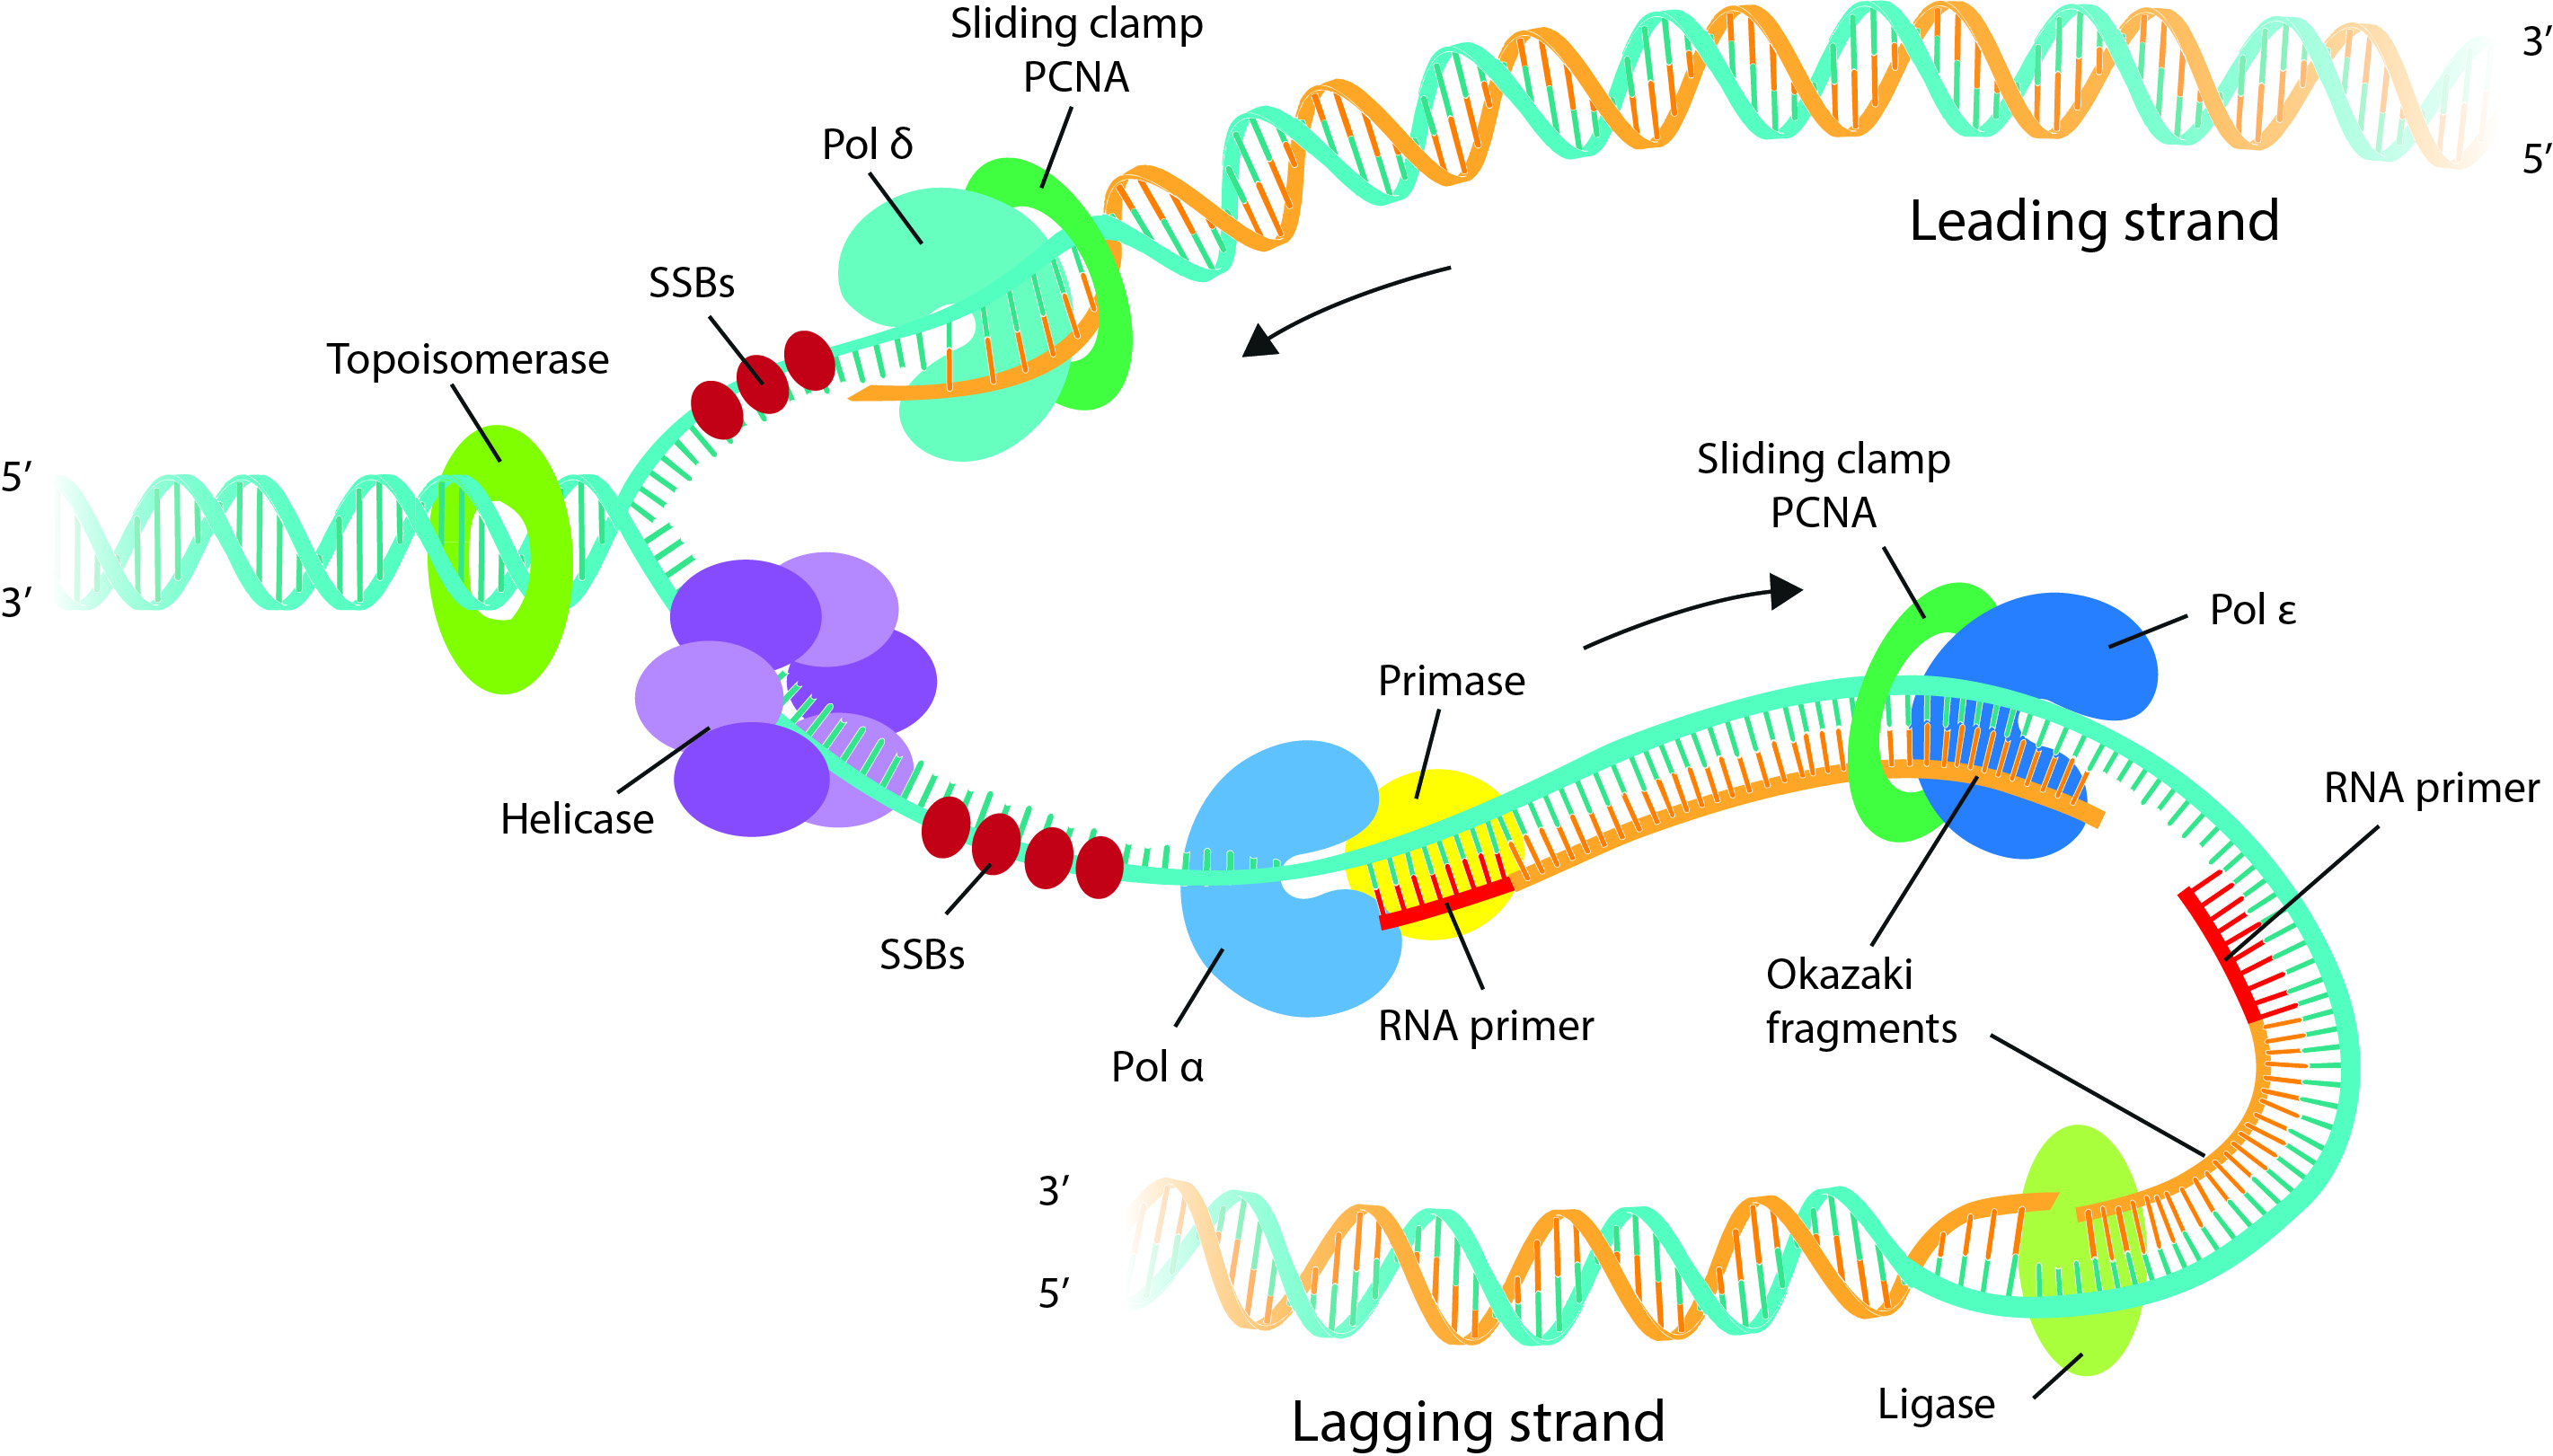
\includegraphics[width=0.85\textwidth]{replication.jpg}
    \centering
    \label{}
\end{figure}


Aby byl systém co nejvýkonnější, dochází k velkému množství replikačních reakcí najednou.

\paragraph{Topoizomeráza}
\begin{myItemize}[nosep]
    \item rozvolní superhelix
\end{myItemize}



\paragraph{Replisom}
\begin{myItemize}[nosep]
    \item vyšší dynamická struktura
    \item sdružuje více proteinů: ORC, helikázu, DNA polymerázu, topoizomerázu
\end{myItemize}



\paragraph{ORC (origin recognition complex)}
\begin{myItemize}[nosep]
    \item trochu DNA ohne, ta je lépe přístupná pro další proteiny (např. helikázy)
    \item ATPáza složená z 6 podjednotek (hexamer)
    \item má specifické vnitřní rozhraní, které rozpozná specifickou sekvenci DNA (až 17 bazí)
    \item často bohatý na AT báze
\begin{myItemize}[nosep]
    \item <= mají slabší vazby a jdou tak lépe oddělit
\end{myItemize}

\end{myItemize}



\paragraph{Helikáza}
\begin{myItemize}[nosep]
    \item rozdělí vlákna DNA, vytvoří replikační vidličku
    \item tvořena dvěma hexamery
\begin{myItemize}[nosep]
    \item na začátku je hexamer otevřený (tvar písmene C) potom se zavře, přistoupí další proteiny, dochází k vlastnímu rozplétání
    \item hexamery na sebe nasedají s posunem, protože jsou mimo osu, na DNA je vyvíjen tlak a začne se rozplétat
\end{myItemize}

    \item např. MCM (minichromosome maintenance protein complex)
\end{myItemize}



\paragraph{DNA polymeráza}
\begin{myItemize}[nosep]
    \item má schopnost tvořit i štěpit DNA
    \item na jednom vlákně vytváří nové vlákno lineárně, na druhém přerušovaně přes okazakiho fragmenty
    \item jeden z nejkonzervovanějších a nejprozkoumanějších proteinů
\end{myItemize}



\paragraph{Topoizomeráza}
\begin{myItemize}[nosep]
    \item přeštípne jeden řetězec, rozmotá jedno překřížení a zase vlákno spojí
\begin{myItemize}[nosep]
    \item za polymerázou dochází k nechtěné torzi (tlačí před sebou otočky DNA), přesně toto řeší TOPOI
\end{myItemize}

    \item ATPáza (potřebuje ATP pro vznik dimeru, tj. k vlastnímu sestřihu)
    \item striktně alfa-helikální struktury
    \item v aktivním místě má Tyr schopné navázat se na báze
    \item existují různé druhy
\begin{myItemize}[nosep]
    \item např TOPOI štěpí jen jeden řetězec a TOPOII štěpí dva
\end{myItemize}

\end{myItemize}



\paragraph{Telomeráza}
\begin{myItemize}[nosep]
    \item polymeráza neumí dojít až na úplný konec vlákna, replikací přicházíme o několik posledních párů bazí
    \item proto jsou na koncích chromozomů telomery s repetitivními sekvencemi
    \item enzym telomeráza je umí doplňovat
\begin{myItemize}[nosep]
    \item nese si vlastní templátovou RNA, podle které ony konce dosyntetizuje
\end{myItemize}

    \item multikomplex proteinové části (enzymatická aktivita) a RNA (templát)
\begin{myItemize}[nosep]
    \item templát: RNA sbalená do pseudoknotu (pevná struktura, chová se jako protein)
\end{myItemize}

\end{myItemize}



\subsection{DNA repair} \label{DNA repair}


\begin{myItemize}[nosep]
    \item při replikaci dochází k mnoha chybám
    \item poškození DNA
\begin{myItemize}[nosep]
    \item chybějící báze
    \item nežádoucí spojování bazí
    \item kovalentně modifikované báze v určitých pozicích
\end{myItemize}

    \item musí existovat řízený opravný mechanizmus
\end{myItemize}



\paragraph{DNA-proteokináza}
\begin{myItemize}[nosep]
    \item strukturní element, který pojme DNA konec a ochrání ho před dalšími reakcemi
    \item má kinázovou doménu
    \item některé části nají tvar solenoidu tvořeného helix-smyčka-helix úseky
    \item rozpozná celý systém
    \item vytvoří synapsi a přivolá další proteiny včetně ligázy
\end{myItemize}



Proteiokináza je na místo potřeby "zavolána" \textbf{KU proteinem}, který našel chybu (break). Přerušené vlákno jsou poté schopny spojit \textbf{ligázy}.

\section{Transkripce} \label{Transkripce} \FloatBarrier


\paragraph{Regulace transkripce}
\begin{myItemize}[nosep]
    \item posttranslační modifikace na histonu
\begin{myItemize}[nosep]
    \item methylace, acylace atd.
    \item jsou k tomu třeba modifikující enzymy (readers, writers, protein 14-3-3)
\end{myItemize}

\end{myItemize}



\paragraph{Kontrolní elementy transkripce}
\begin{myItemize}[nosep]
    \item promotory, enhancery
    \item chromatin v superorientaci
\begin{myItemize}[nosep]
    \item potřebujeme ho remodulovat --- rozvolnit více organizované shluky
\end{myItemize}

    \item enhancery
\begin{myItemize}[nosep]
    \item oblasti DNA, na které se vážou regulační proteiny
    \item na DNA vzniká smyčka, společně s velkým mediátorovým komplexem to má za následek přiblížení enhancerové části a polymerázy
\begin{myItemize}[nosep]
    \item tím páem mohou být enhancery až stovky bazí daleko od vlastního genu
\end{myItemize}

\end{myItemize}

\end{myItemize}



\paragraph{Transkripční faktory}
\begin{myItemize}[nosep]
    \item dokáží rozpoznávat specifické sekvence DNA (promotorové regiony, enhancery)
    \item faktory lze rozdělit podle konformací, které zaujímají
\begin{myItemize}[nosep]
    \item většinou tvoří heterodimery, mají tvar alfa helixu
    \item specifita daná dvěma úseky DNA vedle sebe
    \item motivy
\begin{myItemize}[nosep]
    \item zinc finger
\begin{myItemize}[nosep]
    \item koordinuje zinkové atomy, které drží konformaci v aktivním stavu
\end{myItemize}

    \item leucinový zip
\begin{myItemize}[nosep]
    \item motiv pomocí něhož některé bílkoviny vytvářejí dimery
    \item strany zipu se k sobě koordinují hydrofobními interakcemi
\end{myItemize}

\end{myItemize}

\end{myItemize}

    \item pioneer faktor
\begin{myItemize}[nosep]
    \item umí vázat histonový oktamer
    \item např. faktor FoxA
\begin{myItemize}[nosep]
    \item strukturou se podobá histonu H1
    \item dokáže napodobit interakci H1 přes vazebnou doménu
\end{myItemize}

\end{myItemize}

\end{myItemize}



\paragraph{Eukaryotická transkripce}
\begin{myItemize}[nosep]
    \item polymerázová reakce
    \item RNA polymeráza
\begin{myItemize}[nosep]
    \item v aktivním místě se nalézá \(\ce{Mg}\)
    \item 3 typy, které se liší složením podjednotek a svým účelem
\begin{myItemize}[nosep]
    \item I umí syntetizovat RNA prekurzor
    \item II transkribuje mRNA a malé nekódující RNA
    \item III transkribuje tRNA
\end{myItemize}

    \item regulace pomocí fosforylace nestrukturovaného C konce
\end{myItemize}

    \item přenos polymeráz
\begin{myItemize}[nosep]
    \item vytvoření většího množství komplexů
    \item chaperonové proteiny pomohou jednotkám k přechodu přes nukleární pór do jádra
\end{myItemize}

\end{myItemize}



\subsection{Splicing} \label{Splicing}


\begin{myItemize}[nosep]
    \item vystřižení intronů, spojení exonů
    \item exony jsou různě kombinovány, pre-mRNA může být spliceována více způsoby
    \item začátek a konec intronu, stejně jako místo, kde se má připojit lariát (viz obrázek), mají své typické "konsenzuální" sekvence
\begin{myItemize}[nosep]
    \item tyto sekvence jsou rozpoznány spliceosomem
\end{myItemize}

\end{myItemize}



\paragraph{Spliceosom}
\begin{myItemize}[nosep]
    \item jádro tvořeno snRNP (small nuclear RNA + protein subunit)
    \item snRNP umí rozpoznat signální sekvence na pre-mRNA, které označují introny
\end{myItemize}



\begin{figure}
    \caption{Schéma popisující průběh splicingu}
    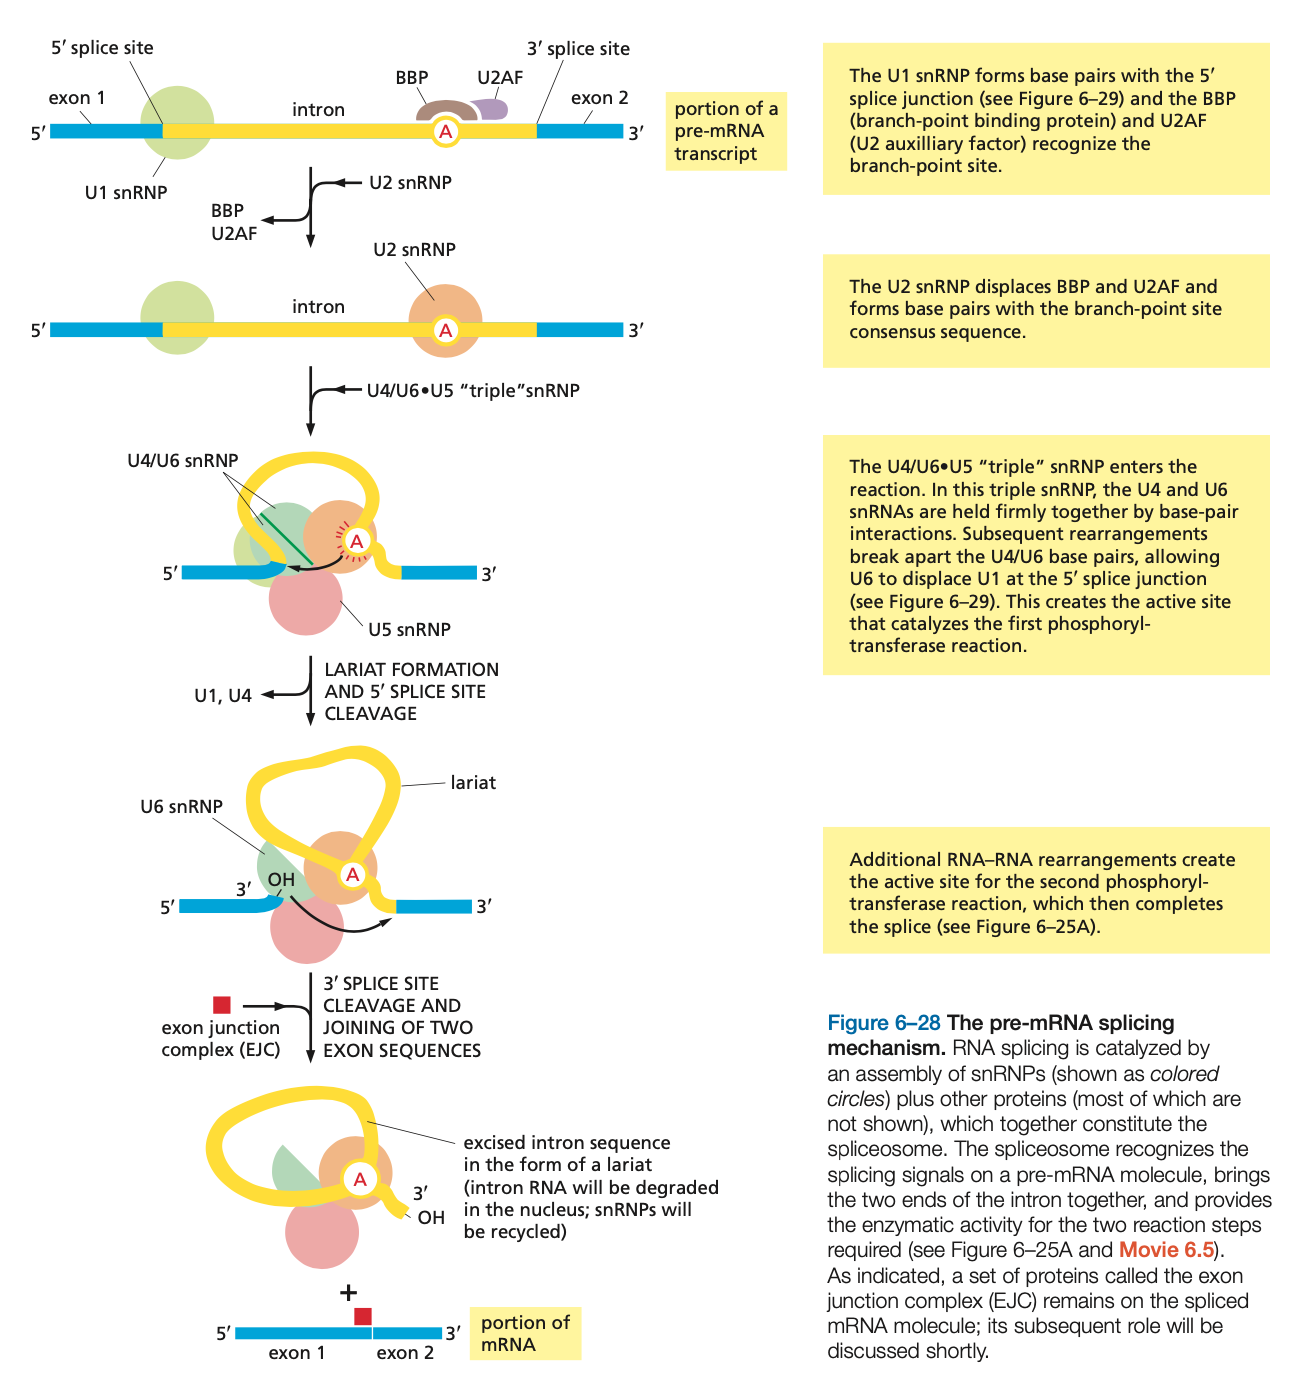
\includegraphics[width=0.85\textwidth]{splicing.png}
    \centering
    \label{}
\end{figure}




\subsection{Chromatine remodeling} \label{Chromatine remodeling}


\begin{myItemize}[nosep]
    \item k DNA na nukleozomech není možné se dostat, je proto nutné chromatin \emph{remodelovat} tak, abychom si DNA mohli přečíst
    \item potřeba dodat ATP
    \item způsoby remodelingu
\begin{myItemize}[nosep]
    \item posunutí nukleozomu
\begin{myItemize}[nosep]
    \item odhalení té části DNA, kterou potřebujeme
    \item velmi energeticky náročné (překonávání elektrostatických interakcí)
\end{myItemize}

    \item zbavení se nukleozomu
\begin{myItemize}[nosep]
    \item díky chaperonům ale zůstává stále poblíž, "naskočí" rychle zpátky
\end{myItemize}

    \item zhušťování a ředění vzdálenosti nukleozomů
    \item výměna histonu (nejčastěji H2)
\end{myItemize}

\end{myItemize}



\paragraph{Fáze}
\begin{myEnumerate}[nosep]
    \item recruitment
    \item ATP depending pumping
    \item uvolnění interakce
    \item pootočen dalšími faktory (může dojít k rozpadu celého nukleozomu)
\end{myEnumerate}



\paragraph{ATP-dependent chromatin remodeling complexes}
\begin{myItemize}[nosep]
    \item známe 4 typy
    \item SWI-SNF family
    \item INO80 family
\begin{myItemize}[nosep]
    \item vícejednotkový
    \item základem je hexamer z proteinů Rvb1/Rvb2
    \item nemá ATPázovou aktivitu
    \item funguje jako stator pro molekulární motor
\begin{myItemize}[nosep]
    \item recyklací ATP je schopen se otáčet
    \item jsou k tomu potřeba další proteiny, které uchopí nukleozom
\end{myItemize}

\end{myItemize}

    \item ISWI family
\end{myItemize}



\section{Translace} \label{Translace} \FloatBarrier


\begin{description}
\item[translace]\hfill \\
Syntéza proteinu na základě informace zakódované v mRNA. Probíhá na ribozomu.

\end{description}


\paragraph{Zainteresovaná RNA}
\begin{myItemize}[nosep]
    \item mRNA
\begin{myItemize}[nosep]
    \item výsledkem transkripce z jádra
    \item transportována z jádra do cytoplazmy
    \item tam je rozpoznána ribozomem a ukotvena
\end{myItemize}

    \item tRNA
\begin{myItemize}[nosep]
    \item struktura trojlístku s rameny (ve 3D tvoří písmeno L)
    \item struktura je konzervovaná, ale s variabilní smyčkou
    \item akceptorové rameno
\begin{myItemize}[nosep]
    \item 3' konec: ACC
    \item váže aminokyselinu
\end{myItemize}

\end{myItemize}

    \item rRNA
\begin{myItemize}[nosep]
    \item tvoří ribozom
\end{myItemize}

\end{myItemize}



\paragraph{Ribozymy}
\begin{myItemize}[nosep]
    \item nukleové kyseliny s katalytickou funkcí
    \item enzymaticky aktivní
    \item umí štěpit cukrfosfátovou kostru
\end{myItemize}



\subsection{Ribozom} \label{Ribozom}


\begin{myItemize}[nosep]
    \item má tři významná místa
\begin{myItemize}[nosep]
    \item A místo, akceptorové místo pro nově přicházející tRNA
    \item T místo, kde se váže tRNA na tvořící se polypeptidový řetězec
    \item E místo, kde prázdná tRNA opouští ribozom
\end{myItemize}

    \item první schéma už z 60.--70. let
    \item 2000 struktur v PDB
\end{myItemize}



\paragraph{Malá podjednotka}
\begin{myItemize}[nosep]
    \item 30S
    \item molární váha 0,85 MD
    \item cca 1600 nukleotidů
    \item 21 proteinů (S1, ..., S21)
    \item odpovídá za rozpoznání
    \item váže se na ni mRNA
    \item dekódování genetické informace
    \item nasedá jako první
\end{myItemize}



\paragraph{Velká podjednotka}
\begin{myItemize}[nosep]
    \item 50S
    \item molární váha 2,5 MD
    \item cca 3000 nukleotidů
    \item 34 proteinů (L1, ..., L34)
    \item dva RNA řetězce
    \item enzym, který vytváří peptidovou vazbu
    \item elongace peptidového řetězce a jeho ochrana
    \item odpovídá za katalýzu peptidové vazby - elongaci
\end{myItemize}



\paragraph{Antibiotika}
\begin{myItemize}[nosep]
    \item řada z nich se váže na ribozom bakterie
    \item zastavují translaci
    \item váží se přímo do aktivního místa
\begin{myItemize}[nosep]
    \item zabraňují vzniku peptidické vazby na tvořícím se proteinu
\end{myItemize}

\end{myItemize}



\subsection{Životní cyklus proteinů} \label{Životní cyklus proteinů}


\begin{myEnumerate}[nosep]
    \item připojení AK na tRNA
    \item syntéza
    \item folding
    \item degradace
\end{myEnumerate}



\paragraph{Připojení AK}
\begin{myItemize}[nosep]
    \item aminoacyl tRNA syntetáza (aaRS)
\begin{myItemize}[nosep]
    \item umí připojit AK na tRNA
    \item dvě vazebná místa (jedno pro tRNA a druhé pro AK)
\end{myItemize}

    \item strukturní variabilita enzymů
\begin{myItemize}[nosep]
    \item velice se liší celkovou strukturou, ale aktivní místo mají všechny skoro stejné
    \item dvě třídy (a několik podtříd)
\begin{myEnumerate}[nosep]
    \item OH skupina na 2' uhlíku
\begin{myItemize}[nosep]
    \item Rosmannův fold (kombinace beta listů a helixů)
    \item aktivní místo na povrchu
\end{myItemize}

    \item OH skupina na 3' uhlíku
\begin{myItemize}[nosep]
    \item antiparalelní beta listy
    \item aktivní místo uvnitř
\end{myItemize}

\end{myEnumerate}

\end{myItemize}

    \item opravy enzymů
\end{myItemize}



Isoleucyl-RS je vyjímka; má dvě ak­tivní mís­ta.
\begin{myItemize}[nosep]
    \item  snaha zaručit, že se místo Ile nenaváže Val, který je Ile tvarem velice podobný
\begin{myItemize}[nosep]
    \item Ile je zpravid­la velice důležitý pro fold­ing pro­teinu
\end{myItemize}

    \item do prvního místa se může navázat Ile nebo Val, do druhého jen Val
    \item pokud se do prvního místa naváže Val, naváže se i do druhého (obě místa jsou blízko sebe)
\begin{myItemize}[nosep]
    \item enzym si toho všimne a Val odštěpí
\end{myItemize}

    \item pokud se do prvního místa naváže Ile, druhé místo zůstane prázdné
\end{myItemize}



\paragraph{Syntéza proteinu}
\begin{myItemize}[nosep]
    \item probíhá na ribozomu
    \item nasednutí malé podjednotky na templát
    \item přicházející tRNA nasedne do T místa ribozomu
    \item přikrytí velkou podjednotkou
    \item další tRNA nasedne do akceptorového místa (EF-Tu protein, "pošťák")
    \item G-faktor tvoří peptidovou vazbu
    \item tRNA odejde a řetězec se posune
\end{myItemize}



\paragraph{Folding proteinu}
\begin{myItemize}[nosep]
    \item jednoduché proteiny se umí sbalit samy
    \item složitější potřebují chaperony, chaperoniny
\begin{myItemize}[nosep]
    \item pomáhají sbalování proteinů, zvlášť těch multidoménových
    \item chaperony jsou monomery, chaperoniny oligomery z chaperonů
    \item např. HSP (heat shock protein)
\begin{myItemize}[nosep]
    \item pozorován při vystavení bakterií vysoké teplotě
\end{myItemize}

    \item GroEL-GroES
\begin{myItemize}[nosep]
    \item bakteriální chaperoniny
    \item HSP 90, HSP 10
    \item dutina na začátku vyplněna hydrofobními AK, tvoří víčko
\begin{myItemize}[nosep]
    \item když se zavře, dutina se zvětší a dochází ke konformačním změnám
    \item do lumen komplexu se dostanou nabité AK
\begin{myItemize}[nosep]
    \item ideální prostředí k foldingu
\end{myItemize}

\end{myItemize}

\end{myItemize}

\end{myItemize}

\end{myItemize}




\paragraph{Degradace proteinů}
\begin{myItemize}[nosep]
    \item když přestanou být potřeba, buňka je recykluje
    \item proteázy
\begin{myItemize}[nosep]
    \item volně putují v cytoplazmě
    \item degradují proteiny
\end{myItemize}

    \item proteasom
\begin{myItemize}[nosep]
    \item velký komplex proteáz
    \item 19S jednotka rozpozná ubiquitinované proteiny a jen ty pustí dovnitř
    \item v centrální části má "mlýnek" (20S jednotka)
\begin{myItemize}[nosep]
    \item štěpí proteiny na krátké úseky (5--7 peptidů)
    \item v cytoplazmě je rozštěpí další proteázy
    \item ubiquitin se recykluje
\end{myItemize}

    \item některé proteasomy berou všechny proteiny co najdou
\begin{myItemize}[nosep]
    \item ukáží je na povrchu
    \item buňky imunitního systému pak mohou rozpoznat infekční proteiny
\end{myItemize}

\end{myItemize}

    \item ubiquitin-proteasome pathway
\begin{myItemize}[nosep]
    \item enzymy ve všech prokaryotech i některých bakteriích kromě archeí
    \item ubiquitin ligáza
\begin{myItemize}[nosep]
    \item připojí ubiquitin s lysiny
    \item jeden ubiquitin nemusí znamenat degradaci
\begin{myItemize}[nosep]
    \item připojují se další, nastane \emph{polyubiquitinace}
\end{myItemize}

\end{myItemize}

\end{myItemize}

\end{myItemize}



\chapter{Přenos signálu v buňce} \label{Přenos signálu v buňce}


\section{Receptory} \label{Receptory} \FloatBarrier


\paragraph{Části}
\begin{myItemize}[nosep]
    \item extracelulární vazebná doména
    \item transmembránová doména
\begin{myItemize}[nosep]
    \item alfa-helikální
    \item "spojka" --- spojuje extracelulární a intracelulární
\end{myItemize}

    \item intracelulární
\begin{myItemize}[nosep]
    \item spojena s enzymatickou funkcí
    \item probíhá sled reakcí, které mohou vést až ke změně genové exprese
\end{myItemize}

\end{myItemize}



\paragraph{Typy}
\begin{myItemize}[nosep]
    \item ligand-gated iontové kanály
\begin{myItemize}[nosep]
    \item reagují na vazbu ligandu otevřením/zavřením
    \item nejrychlejší reakce
\end{myItemize}

    \item receptory spojené s G proteiny
\begin{myItemize}[nosep]
    \item také relativně rychlé
    \item produkují sekundární posly
\end{myItemize}

    \item receptory spojené s kinázami
    \item jaderné receptory
\begin{myItemize}[nosep]
    \item pod membránou
    \item nemají transmembránovou část
    \item ligandem jsou většinou melé hydrofobní molekuly
\end{myItemize}

\end{myItemize}



\subsection{Fosforylace} \label{Fosforylace}


\begin{myItemize}[nosep]
    \item nejběžnější typ posttranslační modifikace
    \item až 13 000 fosforylovaných proteinů, 230 fosforylačních míst
    \item spotřeba ATP/GTP pro přenos fosfátu na protein
    \item reverzibilní proces (fosfatázy)
    \item kinázová doména je dobře konzervovaná
    \item funkce
\begin{myItemize}[nosep]
    \item vytvořit interakci (fosfátová skupina interaguje přes hydroxylovou skupinu) nebo naopak interakci zabránit
    \item spustit enzymatickou reakci
    \item přidání náboje (fosfátová skupina je záporně nabitá)
\end{myItemize}

    \item tyrosinová fosforylace
\begin{myItemize}[nosep]
    \item reader: SH2 doména
\begin{myItemize}[nosep]
    \item rozpoznává tyrosiny
\end{myItemize}

    \item writer: tyrosin kináza
\begin{myItemize}[nosep]
    \item modul, který fosforyluje
\end{myItemize}

    \item eraser: P-Tyr fosfatáza
\begin{myItemize}[nosep]
    \item modul, který defosforyluje
\end{myItemize}

\end{myItemize}

\end{myItemize}



\paragraph{Src kináza}
\begin{myItemize}[nosep]
    \item tyrosin kináza
    \item má unikátní doménové uspořádání
    \item SH4 doména
\begin{myItemize}[nosep]
    \item krátký úsek několika málo AK
    \item slouží k ukotvení do membrány
\end{myItemize}

    \item unique doména
\begin{myItemize}[nosep]
    \item asi 100 AK
    \item neuspořádaná oblast (čili pro ni nemáme strukturu)
\end{myItemize}

    \item SH3 doména
\begin{myItemize}[nosep]
    \item interaguje s SH4 a unikátní doménou (přes dvě smyčky)
    \item polyprolinový helix
\begin{myItemize}[nosep]
    \item výskyt v linkeru
    \item dojde-li k rozvolnění struktury, linker se uvolní do struktury
\end{myItemize}

    \item delece SH3 vede  narušení regulace kinázové aktivity -> leukemie
\end{myItemize}

    \item SH2 doména
\begin{myItemize}[nosep]
    \item asi 100 AK
    \item umí rozpoznat fosforylovaný tyrosin
\end{myItemize}

    \item SH1 doména
\end{myItemize}



\mybox{Poznámka}{Proteiny bez konformace, intrinsically disordered proteins (IDP): více informací například \href{https://eugleo.github.io/bioinformatika/doc/zaklady-bioinformatiky\#Intrinsically disordered proteins}{IDP v zápiscích z bioinformatiky}.

\paragraph{Příklady}
\begin{myItemize}[nosep]
    \item E1A
\begin{myItemize}[nosep]
    \item váže pRB (retinoblastomový protein) a CBP (cap binding proteins)
\end{myItemize}

    \item PKA
\begin{myItemize}[nosep]
    \item fosforylací aktivuje CREB a změní neuspořádané domény KIY v uspořádané
\end{myItemize}

\end{myItemize}

}


\subsection{G-protein-coupled receptors} \label{G-protein-coupled receptors}


\begin{myItemize}[nosep]
    \item rodina eukaryotních proteinů
    \item sedm transmembránových úseků
    \item variabilní ligandy (vůně, neurotransmitery, feromony, hormony, peptidy)
    \item přes 800 genů u člověka (4\% všech protein-kódujících genů)
    \item snad každý fyziologický proces je regulován GPCR
\end{myItemize}



\paragraph{Princip funkce}
\begin{myItemize}[nosep]
    \item na GCPR je navázaný G-protein složený z \(\alpha\) a \(\beta / \gamma\) podjednotek
    \item po navázání ligandu na receptor se z GCPR stane GEF (guanine nucleotide exchange factor), pomůže G\(\alpha\) uvolnit GDP
\begin{myItemize}[nosep]
    \item opačný vliv by měl GAP (GTPase activating protein), který GTPázy inhibuje
\end{myItemize}

    \item uvolněná G\(\alpha\) naváže GTP, změní konformaci, G-protein je uvolněn z receptoru a rozpadá se na dvě části (G\(\alpha\) + G\(\beta / \gamma\))
\begin{myItemize}[nosep]
    \item G\(\alpha\) je tedy GTPáza
    \item obě části se mohou navázat na něco dalšího a tím před signál dál
\end{myItemize}

    \item G\(\alpha\) se vydá k adenylcykláze, která produkuje sekundární posly (cAMP)
\begin{myItemize}[nosep]
    \item cAMP spustí fosfatidyl inositolovou dráhu; její koncentrace se během krátké chvíle může zvýšit až dvacetkrát
    \item proto G\(\alpha\) štěpí GTP (=deaktivuje se) velice rychle; stačí totiž i malá chvíle
\end{myItemize}

\end{myItemize}



\mybox{Poznámka}{Adenylát cykláza má podobný fold jako reverzní transkriptáza a DNA polymeráza (asi společný předek).}


\paragraph{Malé GTPázy}
\begin{myItemize}[nosep]
    \item malé molekuly, kolem 180 AK
    \item molekulární přepínače
    \item schopny fungovat autonomně
    \item ukotvené v membráně
\begin{myItemize}[nosep]
    \item když jsou v membráně, jsou aktivní, a inaktivují se, když se z ní dostanou ven
    \item důsledek konformační změny při navázání GTP/GDP
\end{myItemize}

    \item RAS rodina
\begin{myItemize}[nosep]
    \item Ras
\begin{myItemize}[nosep]
    \item proliferace
    \item často mutovaný v nádorech
    \item účastní se velkého množství drah
    \item SOS protein
\begin{myItemize}[nosep]
    \item při vazbě na Ras způsobí uvolnění navázaného ligandu (urychluje výměnu ligandů)
\end{myItemize}

\end{myItemize}

    \item Rho
\begin{myItemize}[nosep]
    \item morfologie: regulace aktinového cytoskeletu
\end{myItemize}

    \item Rab, Arf
\begin{myItemize}[nosep]
    \item váčkový transport
\end{myItemize}

    \item Ran
\begin{myItemize}[nosep]
    \item jaderný transport
\end{myItemize}

\end{myItemize}

    \item struktura
\begin{myItemize}[nosep]
    \item beta sheet, kolem 3-4 helixy
    \item 2 switche
    \item vyžadují \(\ce{Mg+}\)
\end{myItemize}

\end{myItemize}



\end{document}